\documentclass{report}

\usepackage{graphicx}
\usepackage{listings}
\usepackage{titlesec}
\usepackage{amsmath}
\usepackage{url}
\usepackage{biblatex}
\usepackage[hidelinks]{hyperref}
\usepackage{float}

\addbibresource{references.bib}

\titleformat{\chapter}[display]
  {\normalfont\huge\bfseries}{\chaptertitlename\ \thechapter}{20pt}{\Huge}

\renewcommand{\chaptername}{Task}

\usepackage{inconsolata}

\lstset{
    basicstyle=\ttfamily,
    language=Python, 
    numbers=left,
    frame=lines,
    literate={-}{-}1,
}

\title{ID2090 A4}
\author{Anton Beny M S, ME23B015}
\date{April 2024}
\begin{document}

\maketitle
\newpage

\tableofcontents

\newpage

\chapter{Breaking The Spectre}

\section{Introduction}
This task required us to apply various operations on matrices. The matrix is given as a \texttt{sympy.Matrix} through a YAML serialized file. Moreover, sympy has great built-in functions in order to handle matrices. Therefore, I implemented the solution using the \texttt{sympy} module.

\section{Code}

\subsection{Eigenvalues and Eigenvectors}
The first step was to find the eigenvalues of the given matrix A. Initially, I did it from scratch using \texttt{sympy.roots()}, to solve for $k$ in the characteristic polynomial $k\cdot I - A$, and using \texttt{matrix.nullspace()} to find the eigenvectors. However, this was slow, and therefore the in-built function \texttt{eigenvects()} was used to find eigenvalues and eigenvectors
\newline

\begin{lstlisting}
eigenvalues, eigenvectors = [], []
for eigenvalue, multiplicity, eigenvector in A.eigenvects():
    eigenvalues.extend([eigenvalue] * multiplicity)
    eigenvectors.extend(eigenvector)
\end{lstlisting}

\subsection{Diagonalization}
The next step was to find matrices $\boldsymbol{U}$ and $\boldsymbol{D}$ such that $\boldsymbol{A}=\boldsymbol{U}\boldsymbol{D}\boldsymbol{U}^*$, where $\boldsymbol{U}$ is the Unitary Matrix, and $\boldsymbol{D}$ is the Diagonal Matrix.
\newline

With help from \cite{enwiki:Diagonalization} and \cite{enwiki:Gram_Schmidt}, $\boldsymbol{U}$ and $\boldsymbol{D}$ are found using the following code
\newline

\begin{lstlisting}[caption={Finding $\boldsymbol{U}$ and $\boldsymbol{D}$}]
eigenvectors = sp.GramSchmidt(eigenvectors)
eigenvectors = [v.normalized() for v in eigenvectors]

U = sp.Matrix([eigenvectors])
D = sp.diag(*eigenvalues)
\end{lstlisting}

\subsection{Spectral Decomposition}
Next, we were tasked with finding the spectral decomposition of the matrix. From \cite{enwiki:Eigendecomposition}:

\begin{align}
    \boldsymbol{A} & = \boldsymbol{U}\boldsymbol{D}\boldsymbol{U}^* \notag                                     \\
    \boldsymbol{A} & = \sum_{i=1}^{n}{\lambda_{i} \cdot \boldsymbol{P}_i} \label{eq:spectral_decompostion_sum}
\end{align}

where:
\begin{itemize}
    \item  $n = $ order of matrix $\boldsymbol{A} $ (3 in our case)
    \item $\boldsymbol{P} _{i}=$ the $i^\text{th}$ Projection Matrix
    \item[] \quad \quad It is given by $\boldsymbol{P}_{i} = \boldsymbol{u}_i \cdot \boldsymbol{u}_i ^ {T}$
    \item $u_{i} = $ the $i^\text{th}$ eigenvector, as a column matrix of shape $(n,1)$
    \item $\lambda_{i} = $ the $i^\text{th}$ eigenvalue, as a scalar
\end{itemize}

\begin{lstlisting}[caption={Implementation for Equation \ref{eq:spectral_decompostion_sum}}]
P = {eigenvalue: [] for eigenvalue in eigenvalues}
for eigenvalue, eigenvector in zip(eigenvalues, eigenvectors):
    P[eigenvalue].append(eigenvector * eigenvector.transpose())

spectral_decomposition = None
for eigenvalue in list(P)[::-1]:
    e = sum(P[eigenvalue], sp.zeros(A.shape[0]))
    if spectral_decomposition is None:
        spectral_decomposition = sp.MatMul(eigenvalue, e, evaluate=False)
    else:
        spectral_decomposition = sp.MatAdd(
            spectral_decomposition,
            sp.MatMul(eigenvalue, e, evaluate=False),
            evaluate=False,
        )
\end{lstlisting}

\section{Observations}

Here are a few things that I observed, while working on the Task

\begin{itemize}
    \item The whole field of Matrices (and therefore Linear Algebra) is a vast and deep ocean, and eigenvalues and eigenvectors seem to be a pretty important part of all of that.
    \item \texttt{sympy} has pretty extensive support for matrices and has in-built functions for a lot of operations that can be operated on a given matrix. One example used in the code is \texttt{sp.GramSchmidt()} which tries to orthogonalize a given set of vectors, using the \href{https://en.wikipedia.org/wiki/Gram%E2%80%93Schmidt_process}{Gram-Schmidt} algorithm.
    \item In a case, where the matrix is normal, but has complex eigenvalues, my implementation still works, however, \texttt{sympy.pprint()} has a seizure trying to print the overly complex Projection matrices into a terminal. Using \texttt{IPython.display()}, gives much more readable results. However, it can only be used in a interactive environment such as in a Jupyter Notebook.
\end{itemize}

\section{Conclusion}

\begin{itemize}
    \item I found this task pretty interesting. I have never done anything like this before, and I learnt a lot of new stuff about Matrices throughout the way.
    \item This is the first time I used \texttt{sympy} and I learnt a lot about its capability and functions.
\end{itemize}

\newpage

\chapter{Optimaze}

\section{Introduction}

This is a second-order optimization task, where we have to find first and second order derivatives. Once again, \texttt{sympy} was an obvious choice, because of its extensive support for differential operations such as \texttt{diff()} or \texttt{hessian()}
\section{Code}

\subsection{Initialization}
The first step, was initializing random values to $\boldsymbol{\theta}^0$. For simplicity, it was always chosen to be zero.

\subsection{Criterion}
I chose the criterion to be the following function:
$$\mathcal{L} = \sum_{i = 1}^{N}{\frac{1}{2N}{(a x_i + b y_i + c z_i - 1)^2}}$$

where:
\begin{itemize}
    \item $N = $ total number of points
    \item $a, b, c: $ the components of the normal vector defining the plane.
\end{itemize}

This objective function will be a parabola, but in 3-Dimensional space, which makes it hard to visualize. Nevertheless, this is perfect for our optimization problem, because it would have only one minima (which is the global minima), which occurs when $a, b, c$ are at their optimal values.

\begin{lstlisting}[caption={Declaring the criterion as an expression}]
t1, t2, t3, x, y, z = sp.symbols("t1 t2 t3 x y z")

L = 0.5 * (t1 * x + t2 * y + t3 * z - 1) ** 2
\end{lstlisting}
\subsection{Optimizer}

Because of our neat criterion, any kind of first-degree optimizer such as Gradient Descent, RMSProp, Adam would have also worked. In this problem, we are tasked with using a second order method known as Newton's Steepest Descent method.
\newline

To quote Wikipedia \cite{enwiki:Newtons_method}, which had a simple Geometric Interpretation for Newton's method:

\begin{quote}
    The geometric interpretation of Newton's method is that at each iteration, it amounts to the fitting of a parabola to the graph of $f(x)$ at the trial value $x_{k}$, having the same slope and curvature as the graph at that point, and then proceeding to the maximum or minimum of that parabola.
\end{quote}\label{quote:Newton's method}

The step sizes at time step $t$ is given by $$\Delta\boldsymbol{\theta}^t = (\boldsymbol{H}^{-1})^{t}\boldsymbol{g}^{t}$$

where:
\begin{itemize}
    \item $\boldsymbol{H} = $ Hessian
    \item[] \quad \quad $\boldsymbol{H}_{ij} = \frac{\partial^2 \mathcal{L}}{\partial\theta_i \ \partial\theta_j}$
    \item $\boldsymbol{g} = $ gradient
    \item[] \quad \quad $\boldsymbol{g}_i = \frac{\partial\mathcal{L}}{\partial\theta_i}$
\end{itemize}

And finally, the step is defined as
$$\boldsymbol{\theta}^{t+1} = \boldsymbol{\theta}^{t} - \Delta\boldsymbol{\theta}^t$$

\begin{lstlisting}[caption={Initialization of Gradient and Hessian}]
g = sp.Matrix([L.diff(f"t{_+1}") for _ in range(3)])
H = sp.hessian(L, (t1, t2, t3))
# H = sp.Matrix([[g[_].diff(f"t{__+1}") for __ in range(3)] for _ in range(3)])
\end{lstlisting}\footnote{For simplicity and efficiency, the in-built function to compute Hessian matrix is used. A way to compute Hessian without the in-built function is also presented, but is commented out}

\begin{lstlisting}[caption={A single epoch}, label={code:step}]
sub_theta = {t1: a, t2: b, t3: c}

L_ = L.evalf(subs=sub_theta)
g_ = g.evalf(subs=sub_theta)
H_ = H.evalf(subs=sub_theta)
tL = 0
tg = sp.zeros(3, 1)
tH = sp.zeros(3)

for x1, y1, z1 in points:
    sub_point = {x: x1, y: y1, z: z1}
    tL += L_.evalf(subs=sub_point)
    tg += g_.evalf(subs=sub_point)
    tH += H_.evalf(subs=sub_point)

losses.append(tL)
if early_stop and tL < epsilon:
    break

steps = tH.inv() @ tg

if early_stop and all(abs(step) < epsilon for step in steps):
    break

epochs += 1
a, b, c = (theta - step for theta, step in zip((a, b, c), steps))
\end{lstlisting}

Note that I maintain a list \texttt{losses} that records the loss at each epoch. This will be used in order to plot the losses.
\newline

The code in Listing \ref{code:step} is run at each time step, until:

\begin{itemize}
    \item The loss function falls below a threshold (\texttt{epsilon})
    \item[] \quad \quad \quad \quad OR
    \item All three step sizes fall below a threshold (\texttt{epsilon})
    \item[] \quad \quad \quad \quad OR
    \item A maximum number of iterations is reached
\end{itemize}

\section{Observations}

\begin{itemize}
    \item Newton's method is not used for any real world optimization task because the algorithm requires finding the inverse of the Hessian matrix. In our case, we had 3 variables $(a, b \text{ and } c)$, so the Hessian was a 3 x 3 matrix. However, say if we consider a machine learning model which has tens of thousands (if not millions or billions) of parameters to optimize, finding that many number of double derivatives, and taking the inverse of such a big matrix is not really feasible, as we know that the time complexity for finding the inverse of a $n \times n$ matrix is $\mathcal{O} (n^3)$. Therefore, this method is not used.

          Nevertheless, coming back to our task, we only have three variables to optimize. So, this method is not as computationally expensive.

    \item At first, I was trying to find the optimal values by trying to minimize the perpendicular distance between the plane and the points

          $$\mathcal{L} = \sum_{i = 1}^{N}{\frac{1}{2N}\frac{(ax_i+by_i+cz_i-1)^2}{a^2+b^2+c^2}}$$

          However, this had a problem where instead of doing anything meaningful, the parameters just kept on increasing exponentially. I only explanation that I was able to gather was the fact that at $a\longrightarrow\infty, \ b\longrightarrow\infty, \ c\longrightarrow\infty$: the derivative $\longrightarrow0$, and therefore the optimizer just doubles the values of $a, b, c$ at each step as it thinks that increasing $a, b, c$ will decrease the loss function, although it doesn't and the process repeats.

    \item I noticed that the optimization is always done in a single step (within very low error margins). This agrees with the Geometric interpretation mentioned in \ref{quote:Newton's method}, as the objective function here is quadratic.
          \begin{figure}[H]
              \centering
              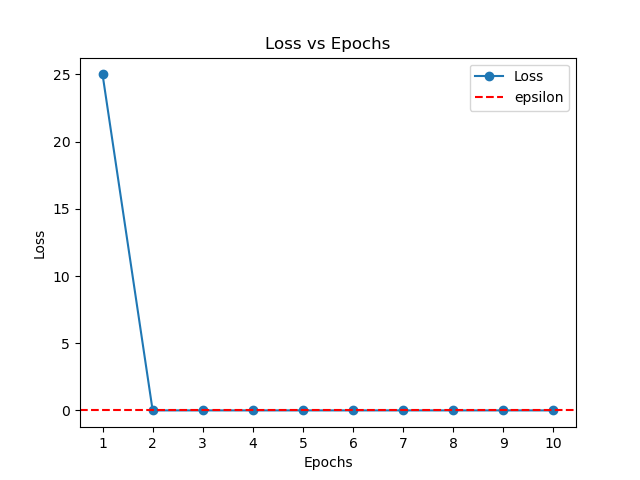
\includegraphics[width=0.5\linewidth]{loss_points.png}
              \caption{A plot of Loss vs Epochs}
              \label{fig:loss_points}
          \end{figure}

          Figure \ref{fig:loss_points} can be better represented by plotting logarithm of losses vs Epochs, as shown here in Figure \ref{fig:logloss_points}
          \begin{figure}[H]
              \centering
              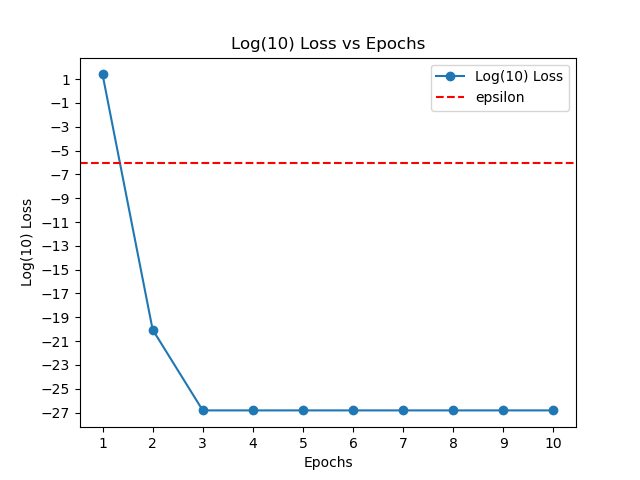
\includegraphics[width=0.5\linewidth]{logloss_points.png}
              \caption{A plot of $log_{10}$ (Loss) vs Epochs}
              \label{fig:logloss_points}
          \end{figure}
          We can see that after the first iteration, the criterion is optimized to a value around $10^{-20}$ which meets the condition that the objective function falls below the threshold $\text{epsilon} = 10^{-6}$.

    \item The given points and the optimal plane is shown in Figure \ref{fig:plane}.
          \begin{figure}[H]
              \centering
              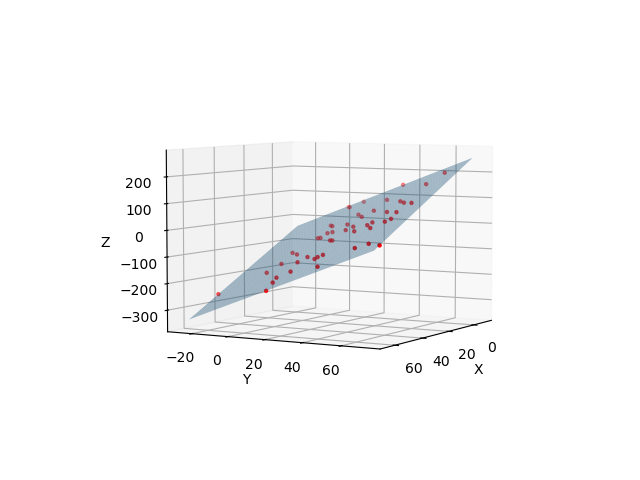
\includegraphics[width=0.5\linewidth]{3d_points.png}
              \caption{A 3-D view of the Points and the Plane}
              \label{fig:plane}
          \end{figure}
\end{itemize}

\section{Conclusion}

\begin{itemize}
    \item I had some prior experience with optimization tasks before, but they were usually simpler, such as Gradient Descent which is a first order method. But this took it to the next level. I learnt a lot of new techniques, especially about second order optimization.
    \item It was a fun experience to discuss and plot different objective functions to determine an efficient one. In the end, I just used the simplest one, sum of squares of algebraic distances.
    \item Once again I was impressed by the capability of the \texttt{sympy} module, which made the implementation for these tasks much simpler.
\end{itemize}

\printbibliography
\end{document}
